\documentclass[compress,aspectratio=169]{beamer}

%%%%%%%%%%%%%%%%%%%%%%%%%%%%%%%%%%%%%%%%%%%%%%%%%%%%%%%%%%%%%%%%%%%%%%%%%%%%%%%
% Packages & theme
%%%%%%%%%%%%%%%%%%%%%%%%%%%%%%%%%%%%%%%%%%%%%%%%%%%%%%%%%%%%%%%%%%%%%%%%%%%%%%%

\usepackage{silence}

\usepackage{luatex85}

\usepackage{hyperref}

\usepackage{graphicx}
\usepackage{epstopdf}
\usepackage{caption}

\usepackage{amsmath}
\usepackage{amssymb}
\usepackage{gensymb}
\usepackage{textcomp}

\usepackage{array}
\usepackage{multirow}
\usepackage{pbox}
\usepackage{multicol}

\usepackage{tabularx,ragged2e}
\usepackage{booktabs}

\usepackage{multimedia}

\usepackage{xstring}

\usetheme{hri}

\usepackage{dtk-logos} % must be loaded after theme
\usepackage{tikz}
\usetikzlibrary{mindmap,backgrounds,positioning}

\graphicspath{{./figures/}{../figures/}}

%%%%%%%%%%%%%%%%%%%%%%%%%%%%%%%%%%%%%%%%%%%%%%%%%%%%%%%%%%%%%%%%%%%%%%%%%%%%%%%
% Settings & Documentwise Variables
%%%%%%%%%%%%%%%%%%%%%%%%%%%%%%%%%%%%%%%%%%%%%%%%%%%%%%%%%%%%%%%%%%%%%%%%%%%%%%%

\newcommand{\presentationtitle}{Title Here}
\newcommand{\presentationsubtitle}{Short Title Here}
\newcommand{\presentingauthor}{Author Author}
\newcommand{\presentationdate}{01.01.3000}
\newcommand{\authorlist}{Author Author, Author2 Author2}
\newcommand{\labname}{Laboratory/Group Name}
\newcommand{\papersubject}{Subject Here}
\newcommand{\paperkeywords}{Keywords Here}

\setbeamertemplate{bibliography item}[text]
\IfStrEq{\jobname}{\detokenize{notes}}{\setbeameroption{show only notes}}{\setbeameroption{hide notes}}

\hyphenation{op-tical net-works semi-conduc-tor}

%Bold face
\renewcommand{\b}[1]{{\Medium #1}}

%Zero left margin
\makeatletter
\newlength\beamerleftmargin
\setlength\beamerleftmargin{\Gm@lmargin}
\makeatother
\newcommand{\zeroleftmargin}{%
	\hspace*{-\beamerleftmargin}%
}

%%%%%%%%%%%%%%%%%%%%%%%%%%%%%%%%%%%%%%%%%%%%%%%%%%%%%%%%%%%%%%%%%%%%%%%%%%%%%%%
% PDF metadata
%%%%%%%%%%%%%%%%%%%%%%%%%%%%%%%%%%%%%%%%%%%%%%%%%%%%%%%%%%%%%%%%%%%%%%%%%%%%%%%

\hypersetup{
	pdftitle={\presentationtitle},
	pdfauthor={\authorlist},
	pdfsubject={\papersubject},
	pdfkeywords={\paperkeywords},
}

\title{\presentationtitle}
\subtitle{\presentationsubtitle}
\date{\presentationdate}
\author{\presentingauthor}
\institute{\labname}

%%%%%%%%%%%%%%%%%%%%%%%%%%%%%%%%%%%%%%%%%%%%%%%%%%%%%%%%%%%%%%%%%%%%%%%%%%%%%%%
% Actual document
%%%%%%%%%%%%%%%%%%%%%%%%%%%%%%%%%%%%%%%%%%%%%%%%%%%%%%%%%%%%%%%%%%%%%%%%%%%%%%%

\begin{document}

\maketitle

%%%%%%%%%%%%%%%%%%%%%%%%%%%%%%%%%%%%%%%%%%%%%%%%%%%%%%%%%%%%%%%%%%%%%%%%%%%%%%%
\section*{Motivation \& Overview}

\begin{frame}{Background \& our motivation}
	\begin{itemize}
		\item Why are we doing this? \cite{example}
	\end{itemize}

	\note{
		\begin{itemize}
			\item Notes about our motivations...
		\end{itemize}
	}
\end{frame}

\begin{frame}
	\frametitle{Table of contents}
	\tableofcontents
\end{frame}

%%%%%%%%%%%%%%%%%%%%%%%%%%%%%%%%%%%%%%%%%%%%%%%%%%%%%%%%%%%%%%%%%%%%%%%%%%%%%%%
\section{Introduction}

\begin{frame}{Introduction}
	\begin{itemize}
		\item What is the problem?
	\end{itemize}

	\note{
		\begin{itemize}
			\item Notes about the problem statement...
		\end{itemize}
	}
\end{frame}

%%%%%%%%%%%%%%%%%%%%%%%%%%%%%%%%%%%%%%%%%%%%%%%%%%%%%%%%%%%%%%%%%%%%%%%%%%%%%%%
\section{Methodology}

\begin{frame}{Methodology}
	\begin{itemize}
		\item What did we do?
	\end{itemize}

	\note{
		\begin{itemize}
			\item Notes about our methodology...
		\end{itemize}
	}
\end{frame}

%%%%%%%%%%%%%%%%%%%%%%%%%%%%%%%%%%%%%%%%%%%%%%%%%%%%%%%%%%%%%%%%%%%%%%%%%%%%%%%
\section{Results}

\begin{frame}{Results}
	\begin{itemize}
		\item What did we learn?
	\end{itemize}

	\note{
		\begin{itemize}
			\item Notes about our results...
		\end{itemize}
	}
\end{frame}

\begin{frame}{Video}
	Here's an example video (go to presentation mode to play):
	\movie[width=0.744\paperheight,height=0.6\paperheight,showcontrols=true,autostart,loop]
        {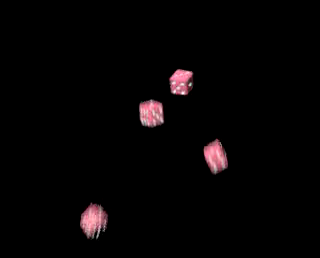
\includegraphics[height=0.6\paperheight]{random-mp4-snapshot}}
        {videos/random.mp4}

	\note{
		\begin{itemize}
			\item Notes about this video...
		\end{itemize}
	}
\end{frame}

\begin{frame}{Zero Left Margin}
	\zeroleftmargin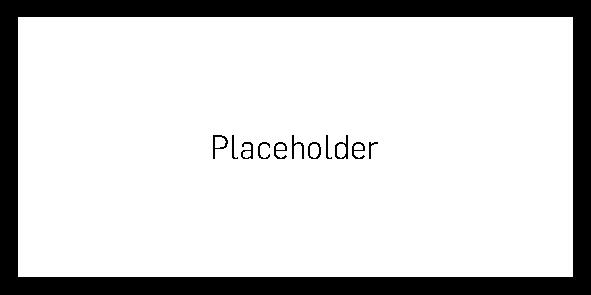
\includegraphics[width=\paperwidth]{placeholder}

	\note{
		\begin{itemize}
			\item This is a frame with exactly zero margin for big images or videos
		\end{itemize}
	}
\end{frame}

%%%%%%%%%%%%%%%%%%%%%%%%%%%%%%%%%%%%%%%%%%%%%%%%%%%%%%%%%%%%%%%%%%%%%%%%%%%%%%%
\section{Conclusion}

\begin{frame}{Conclusion \& future work}
	\begin{itemize}
		\item We will revolutionize the world...
	\end{itemize}

	\note{
		\begin{itemize}
			\item Notes about the conclusion...
		\end{itemize}
	}
\end{frame}

\begin{frame}{Questions \& references}
	\begin{center}
		\LARGE
		Thank you for listening!\\ \vspace{10pt}Questions?
	\end{center}

	\IfStrEq{\jobname}{\detokenize{notes}}{
		%Nothing
	}{
		\fontsize{7pt}{8.4}\selectfont
		\bibliographystyle{plain}
		\bibliography{../../references}
	}
\end{frame}

\end{document}

%%%%%%%%%%%%%%%%%%%%%%%%%%%%%%%%%%%%%%%%%%%%%%%%%%%%%%%%%%%%%%%%%%%%%%%%%%%%%%%
%%%%%%%%%%%%%%%%%%%%%%%%%%%%%%%%%%%%%%%%%%%%%%%%%%%%%%%%%%%%%%%%%%%%%%%%%%%%%%%
%%%%%%%%%%%%%%%%%%%%%%%%%%%%%%%%%%%%%%%%%%%%%%%%%%%%%%%%%%%%%%%%%%%%%%%%%%%%%%%

%Custom background image
% \subsection{Subsection Name}{
% \fullbackground{fullscreen-background-image.jpg}
% \begin{frame}{Fullscreen picture/graphic}
%     \textcolor{white}{
%     Normal text goes here.\cite{example}
%     }
%     \begin{block}{Block with tile}
%         \begin{itemize}
%             \item Item 1
%             \item Item 2
%         \end{itemize}
%     \end{block}
% \end{frame}
% }

%Fullscreen image slide
% \imageframe[What is the image about?]{fullscreen-background-image.jpg}

%TikZ mindmap
% \begin{frame}{Mindmap with TikZ}
% \centering
% \begin{tikzpicture}[scale=0.88]
% 	%\tikzset{every child/.append style={level distance=250}}
% 	\path[mindmap,concept color=hriWarmGreyLight,text=hriWarmGreyDark]
% 	node[concept] {\TeX}
% 	[clockwise from=-30]
% 	child[concept color=hriSec2Dark,text=white] { node[concept] {\textcolor{white}{\XeTeX}} }
% 	child[concept color=hriSec1CompDark,text=white] { node[concept] {\ConTeXt} }
% 	child[concept color=hriSec1Dark,text=white] { node[concept] {\LaTeX} };
% \end{tikzpicture}
% \end{frame}

%Example TikZ figure
% \begin{frame}{TikZ figure}
% 	\begin{figure}
% 		\centering
%
% \resizebox{\paperwidth}{!}{%
%
% \tikzset{subpart/.style={draw, font=\scriptsize, fill opacity=0.5, text opacity=1, fill=white!50}}
%
% \begin{tikzpicture}[
%     >=latex,
%     every edge/.style={draw, very thick},
%     skill/.style={draw, rounded corners, align=center, inner sep=5pt, fill=black!20},
%     label/.style={midway, align=center, font=\scriptsize, fill=white}]
%
%   %%% ORO
%     \node at (0,0)[skill, ultra thick, fill=hriSec2Dark!50] (oro) {{\sc Oro} -- Symbolic facts \\ and beliefs management};
%
%   %%% HATP
%   \node at (-6, 2.5)[skill, fill=hriSec1!50] (hatp) {HATP -- Human-aware \\ symbolic task planning};
%
%   %%% DIALOGS
%   \node at (-6, -3) [skill, fill=hriSec3Dark!50] (dialogs) {{\sc Dialogs} \\ Dialogue processing};
%
%   %%% SPARK
%   \node at (4,-3.5)[skill, fill=hriSec3!50] (spark) {%
%       \begin{tikzpicture}
%           \node at (0,0) (geom) {{\sc Spark} -- Geometric \& Temporal Reasoning};
%         \node [subpart, below=0.2 of geom.south west, anchor=north west] (world-update) {Sensors fusion};
%         \node [subpart, right=0.2 of world-update] (geom-model) {Geometric model of the environment};
%         \node [subpart, right=0.2 of geom-model] (fact-prod) {Symbolic facts production};
%       \end{tikzpicture}
%     };
%
%   %%% MHP
%     \node at (9,0)[skill, fill=hriSec3CompDark!50] (mhp) {{\sc mhp} -- Human-aware \\ Motion and Manipulation \\ Planning};
%
%   %%% SHARY
%   \node at (4,4.5)[skill, fill=hriSec1Comp!50] (shary) {%
%       \begin{tikzpicture}
%         \node at (0,0) (exec) {Execution Controller};
%         \node [subpart, below=0.2 of exec.south west, anchor=north west] (plans) {Goal \& Plans \\ management};
%         \node [subpart, right=0.2 of plans] (sit-asses) {Situation assessment \\ and context management};
%         \node [subpart, right=0.2 of sit-asses] {Action instantiation, \\ execution and monitoring};
%       \end{tikzpicture}
%     };
%
%
%   %%% LOWLEVEL
%   \node [skill, below=0.7 of spark] (lowlevel) {%
%       \begin{tikzpicture}
%         \node at (0,0) (sensori) {Sensorimotor layer};
%         %\node [subpart, below=0.2 of sensori.south west, anchor=north west, align=left] (perception) {{\bf Perception} \\ 2D markers, RGB-D, motion capture};
%         %\node [subpart, align=right, right=0.2 of perception] {{\bf Actuation} \\ Head's pan-tilt unit, grippers, arms, wheels};
%       \end{tikzpicture}
%   };
%
%   %%% Separation between deliberative layer and sensori-motor layer
%   \draw[dotted, thick] (-8,-5) -- (12, -5);
%
%   %%% Relations between components
%   \path (shary.340) edge [<->, bend left] node[label] {motion plan \\ requests} (mhp);
%   \path (shary.west) edge [<->, bend right] node[label] {shared \\ plans} (hatp);
%   \path (hatp) edge [<->, bend right] node[label] {world model and \\ agents beliefs} (oro.170);
%   \path (dialogs) edge [<->, bend left] node[label] {natural language \\ grounding} (oro.190);
%   \path (spark.100) edge [->, bend right] node[label] {symbolic \\ facts} (oro);
%   \path (spark.5) edge [->, bend right] node[label] {environment\\model} (mhp);
%   \path (shary) edge [<->, bend left] node[label] {events, \\ world model and \\ agents beliefs} (oro);
%   \path (shary) edge [<->, bend left] node[label] {action monitoring \\ and management of \\ position hypotheses} (spark);
%   \path (lowlevel) edge [->] (spark);
%   \path (lowlevel.east) edge [<-, bend right=80, looseness=1.5] node[label] {atomic\\actions} (shary.east);
%
% \end{tikzpicture}
% }
% 	\end{figure}
% \end{frame}
